\documentclass{article}
% translate with >> pdflatex -shell-escape <file>

% This file is used as unit test for pgfplots, copyright by Christian Feuersaenger.
% 
% See
%   http://pgfplots.sourceforge.net/pgfplots.pdf
% for pgfplots.
%
% Any required input files (for <plot table> or <plot file> or the table package) can be downloaded
% at
% http://www.ctan.org/tex-archive/graphics/pgf/contrib/pgfplots/doc/latex/
% and
% http://www.ctan.org/tex-archive/graphics/pgf/contrib/pgfplots/doc/latex/plotdata/

\usepackage{pgfplots}
\pgfplotsset{compat=newest}

\pagestyle{empty}

\begin{document}

	Here is a regression -- and it seems as if some spacing parameters between the `$-$` and the $5$ have changed !? It is not in \verb|\pgfmathprintnumber|...

	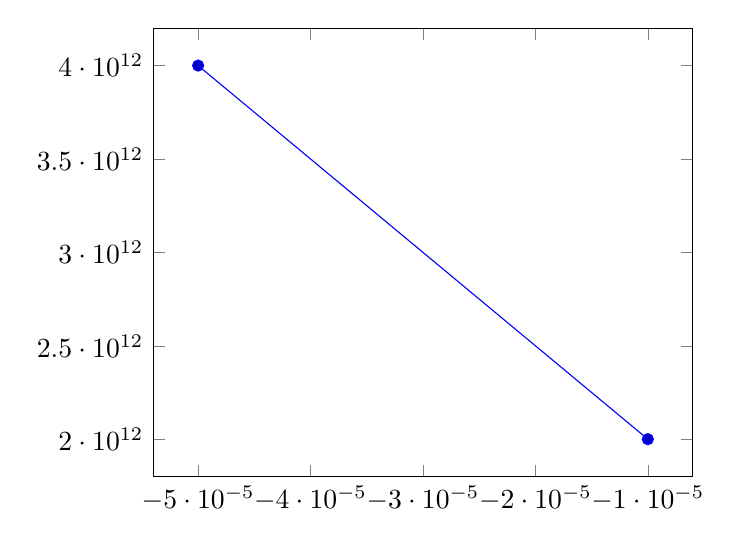
\begin{tikzpicture}
		\begin{axis}[scaled ticks=false]
		\addplot coordinates {(-0.00001,2e12) (-0.00005,4e12) };
		\end{axis}
	\end{tikzpicture}

	\fbox{\pgfmathprintnumber{-0.00005}}

	\fbox{\pgfmathprintnumber{-5e-5}}

	\fbox{\pgfmathprintnumber{-5.00001e-5}}

	\fbox{\pgfmathprintnumber{-4.99999e-5}}
\end{document}
